% Chapter 4
% add following line for typesetting from subfiles
% !TeX root = ../uet_thesis.tex
% !TeX root = ../uet_thesis.bbl
% !TeX root = ../references.bib
\chapter{Power Spectral Density Analysis of Proposed VR-MPPM} % Write in your own chapter title
\label{Chapter4}
\lhead{Chapter 4. \emph{Power Spectral Density Analysis}} % Write in your own chapter title to set the page header
%\section{Introduction}


%
%4)	PSD Analysis of proposed code
%i)	Method for PSD analysis
%(a)	Spectra Calculation by 1)Bosik 2) Cariolaro: 
%(b)	Ergodicity and wide sense stationarity
%b)	Statelessness of VR-MPPM: Simplifies PSD Analysis
%i)	Equations simplification for MPPM case
%(a)	PSD analysis of a simple case (n=4, BI=.25,  = .25)
%ii)	Implementation
%(a)	MPPM PSD cases: graphs
%(b)	Matlab code
%iii)	PSD Observations
%(a)	Strong spectral component at bit frequency: clock extraction
%(b)	DC component verifies intuition

Power spectral density (PSD) analysis of a signal provides important information about the signal characteristics that help in optimal system design. For that reason the power spectral density analysis of the proposed VR-MPPM encoded signal is being presented here.

Spectral characteristics of a signal determine to a large extent the system complexity. Parameters like bandwidth requirements, presence of adequate frequency components for clock extraction and absence of DC null determine the effectiveness and feasibility of a line code.

Generally codes with smaller bandwidth requirements are preferred over the ones that need larger bandwidth. It is also a desired feature for a line code to have strong spectral component at clock frequency for transmitter-receiver synchronization. Digital line coding schemes like Manchester and Bipolar encoding were designed especially with that purpose in mind. PSD analysis of the proposed VR-MPPM would determine whether or not it is a self clocking code. DC null is a preferred feature in digital signalling. A DC biased signal tends to saturate the capacitive and inductive couplings in the system which preform best with AC signals. Therefore a strong DC bias creates problems in signal reconstruction at digital line repeaters and regenerators along the transmission. In optical transmission networks this requirement can be somewhat relaxed as optical signal is DC signal by its very nature. Optical receivers operate on photon counting principle for pulse detection in this DC biased signal. This is one of the reasons for widespread use of PPM and its variants in optical transmission. The proposed VR-MPPM scheme possesses a strong DC component at all code rates and it determines the brightness level of the visible light communication transmitter. In optical broadcasting systems, such as visible light communication, the need for signal regeneration is not that much of an importance as transmitter and receiver operated in close vicinity. It means that the requirement of DC null for the line code needs to be relaxed in our case.

PPM transmits information by position of a pulse in the symbol frame. Therefore DC average of  the signal remains constant, irrespective of the information bits being transmitted. Same is the case for VR-MPPM encoding with a small difference that DC bias remains constant for a selected brightness level but changes when the brightness level is changed to a new value according to the illumination needs. In a practical situation the requirement of brightness change is not so frequent and may need to be changed after time periods much more longer than the symbol time. Therefore to evaluate the spectral properties of proposed codes it is supposed that the transmitter is set at a certain brightness level that remains constant over infinite time to fulfil  theoretical requirement. The spectral density would be calculated for a fixed frame size and at a particular brightness level.

\section{Signal Stationarity}

The data transmitted by an information source is a random process by its nature. As a result the line code carrying this information is also a random signal. A random process is  categorized as a power signal, that is a signal with finite power.

The proposed VR-MPPM scheme is essentially a blockcode which takes an M-bit input symbol and maps it to a codeword of N bits. This (M,N) block encoder is depicted in figure \ref{block_encoder}. The encoder that performs this mapping is a memoryless system. It means that the encoded output for a symbol remains constant irrespective of its position in the input data stream. Because input bit stream is a random or stochastic process, so is the output signal at encoder output. The statistical properties of the encoder output are function of both the statistical properties of the input symbol sequence and the statistics of the encoder itself. 

\begin{figure}
	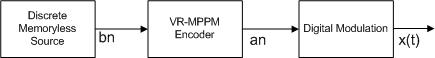
\includegraphics[width=\textwidth]{./Figures/block_encoder}
	\caption{Encoder block diagram}
	\label{block_encoder}
\end{figure}

The PSD of a stochastic process can not be evaluated directly from Fourier Transform due to non-deterministic nature of the signal. In this situation Einstein-Wiener-Khintchine help with a relationship between power spectral density and auto correlation function of a random process, mathematically expressed by equation \ref{eq:wkSx} and equation \ref{eq:wkRx}.

\begin{equation}
	S_x(f)=\int_{-\infty}^{\infty}R_x(\tau)~e^{-j 2 \pi f \tau} d\tau
	\label{eq:wkSx}
\end{equation}

\begin{equation}
	R_x(\tau)=\int_{-\infty}^{\infty}S_x(f)~e^{j 2 \pi f \tau} df
	\label{eq:wkRx}
\end{equation}

The equation \ref{eq:wkSx} possesses special importance as it allows to evaluate PSD of a signal from its autocorrelation function $R_x$. The necessary condition for this relationship to be useful is that the signal should be stationary. That is its statistical properties should not change over time. For communication signals it is enough if the signal meets the two wide sense stationarity criterion given in equations \ref{eq:cond1} and \ref{R_x_t1_t2}.

\begin{equation}
	E\{X(t)\}=\mu_x = Constant
	\label{eq:cond1}
\end{equation}

Where $E\{\cdot\}$ is the expectation operator and $X(t)$ is the random variable for the stochastic process. This equation expresses that the signal mean value should remain constant over time.

\begin{equation}
	R_x(t_1,t_2)=R_x(t_1-t_2)
	\label{eq:cond2}
\end{equation}

The equation \ref{eq:cond2} states that the autocorrelation function should be a function of only the time difference and should not be dependant on absolute time. Therefore $t_1-t_2$ in \ref{eq:cond2} may be replaced by $\tau$, giving $R_x(\tau)=R_x(t_1-t_2)$. It can be evaluated as:

\begin{equation}
	R_x(\tau)=E\{X(t) X(t+\tau)\}
	\label{R_x_t1_t2}
\end{equation}

In our case it is a reasonable assumption that the information source transmits all symbols with equal probabilities and these probabilities do not change over time. It implies that the signal mean and autocorrelation function remain constant with time shift. This satisfies the above mentioned signal widesense stationarity criterion. Since the encoder simply translates input symbols to output codes without memory, encoder output code word sequence also constitute a widesense stationary process. However the encoder output bit sequence is a cyclostationary process \cite{cariolaro1974spectra} with period $N\cdot T_b$, where $T_b$ is the bit period and $N$ is the number of bits per codeword.
%

\section{Spectral Density Formula}
Power spectral density analysis of block coded signals is investigated by several authors. The technique proposed by \cite{cariolaro1974spectra} is the one that will be used for analysis of VR-MPPM block coded signals. However some simplifications of \cite{cariolaro1974spectra} are required to adopt this technique to our case that are listed in table \ref{tab:simplifications}.

%\begin{table}[hbtp]
\begin{table}[htbp]
\begin{center}
\caption[Assumptions for PSD analysis]{Simplifications from \cite{cariolaro1974spectra} technique for analysis of VR-MPPM block coded signals}
\begin{tabular}{|c|c|}
\hline\hline
General Conditions & Simplification for VR-MPPM\\
\hline\hline
\parbox{2.5in}{
\begin{list}{}{}
\item L-step multilevel line code used to encode symbols 
\item Encoder output is a function of code state and input symbol 
\item	Input symbols arrive with any random probability 
\end{list}
}
 & 
\parbox{2.5in}{
\begin{list}{}{}
\item Binary level line code that with signal level 0 or 1
\item Memoryless system that directly maps input symbols to output codeword
\item   All input symbols are assumed to be equally probable 
\end{list}
}\\
%--&--\\
\hline
\end{tabular}

\label{tab:simplifications}
\end{center}
\end{table}

%        L-step multilevel line code used to encode symbols 
%     Binary level line code that with signal level 0 or 1 \\
%	Encoder output is a function of code state and input symbol 
% Memoryless system that directly maps input symbols to output codeword \\
%	Input symbols arrive with any random probability 
%   All input symbols are equally probable 
%	

%>>>>>>>>>>>>>>>>>>>>>>>>>>>>>>>>>>
%   Letter Freq Analysis
%<<<<<<<<<<<<<<<<<<<<<<<<<<<<<<<<<<
%Generally, each codeword of an encoded message is considered to be a random variable and the resulting sequence of codewords constitute a stochastic process. Statistics of sequence of codewords depend on both the statistics of input symbols as well as on the encoding specifications. 



The spectrum analysis starts from representing the encoded signal waveform by its time domain representation. The modulator output signal consists of a pulse train, with certain pulses grouped in blocks or frames. Often the terms slot and bit will be used interchangeably. A bit is the binary value of a symbol in the encoder output codeword in a frame of $n$ bits. This bit is represented by the symbol $s_i^{(j)}$ so that $i$ indexes the frame in the infinite sequence of codewords and $j$ indexes the individual bit within that frame. These bits are modulated by some form of pulse in the time domain. For its simplicity and easier generation in digital systems, we consider the basic rectangular non-return-to-zero (NRZ) pulse shape $p(t)$ as defined by equation \ref{eq:pulseShape}. 

\begin{equation}
\label{eq:pulseShape}
p(t) = \left\{ \begin{array}{cl}
						1&\frac{-T_b}{2} \leq t \leq \frac{T_b}{2} \\
						0&otherwise
						\end{array}
						\right..
\end{equation}

PSD of this NRZ rectangular pulse is provided by equation \ref{eq:spectrumOfRectPulse}. As this term is multiplied to the continuous and discrete spectral components of the encoder frequency spectrum, it determines the overall envelope. For rectangular pulse the spectrum shape decays with higher frequencies according to the $sinc$ function.

\begin{equation}
\label{eq:spectrumOfRectPulse}
 2 T_b \left[\frac{\sin(2\pi f T_b)}{2\pi f T_b}\right]^2
\end{equation}


The frame time, represented by $T_n$, is defined as $T_n=n\cdot T_b$. The resulting continuous time optical signal is given by equation \ref{eq:xt} 

\begin{equation}
\label{eq:xt}
    x(t) = \sum_{i= - \infty}^{\infty} \sum_{j=1}^n s_i^{(j)} p(t- (j-1)T_b - iT_n)
\end{equation}
The power spectral density $S_x(f)$ of a general linear block code is expressed by the following relation \cite{cariolaro1974spectra}

\begin{equation}
S_x(f) = f_n |P(f)|^2 \left\{  \sum_{k=-\infty}^{\infty} e^{ -j \omega k T_n}~ \mathbf{VR_k V^*} \right\}
\label{eq:spectrum_eq1}
\end{equation}
Where $P(f)$ is the Fourier transform of the pulse shape $p(t)$ used for the line code and $f_n=\frac{1}{T_n}$ is the frame repetition frequency. The vector function $\mathbf{V}$ consisting of exponentials terms defined as:

\begin{equation}
	\mathbf{V}= \left[\mathbf{e}^{j\omega T_b}, \mathbf{e}^{j\omega 2T_b}, \cdots,\mathbf{e}^{j\omega nT_b}\right]
\label{eq:vectorV}
\end{equation}

Its complex conjugate transpose $\mathbf{V^*}$ is given by:
\begin{equation}
	\mathbf{V^*}=
		\left[
		\begin{array}{l}
		\mathbf{e}^{-j\omega T_b} \\
		\mathbf{e}^{-j\omega 2T_b} \\
		\cdots \\
		\mathbf{e}^{-j\omega nT_b}
		\end{array}
		\right]
\end{equation}

The parameter $R_k$ is the code correlation matrix defined by equation \ref{eq:corrCoef}.
\begin{eqnarray} \label{eq:corrCoef}
 R_k &=& 
\begin{array}{lc}
   E[\mathbf{s}_i^{T}, \mathbf{s}_{i+k}]  &  -\infty  < k < \infty
\end{array} \nonumber \\
			&=& \mathbf{S}^T \mathbf{P}_k \mathbf{S}
\end{eqnarray}

Where $E[.]$ is the expectation operator and $\mathbf{S} = [\mathbf{s}_1, \mathbf{s}_2, \cdots, \mathbf{s}_m]$ is the codeword translation matrix.  $\mathbf{P}_k$ is the joint probability matrix between any two codewords $\mathbf{s}_{i}$ and $\mathbf{s}_{i+k}$ that occur in the infinite series of codewords that are set apart by $k$ frames.

\cite{cariolaro1974spectra} has presented another expression for the PSD in terms of continuous and discrete power spectra by equation \ref{eq:spectrum_eq2}. This new form is easier to evaluate on digital computers.

\begin{equation}
    S_x(f) = f_n |P(f)|^2 \left\{X_c(f) + f_n X_d(f) \sum_{k=-\infty}^{\infty} \delta (f - k f_n) \right\}
\label{eq:spectrum_eq2}
\end{equation}

Here $X_c(f)$ is the continuous component of the signal spectrum given by 
\begin{equation} 
\label{eq:contSpec}
    X_c(f) =\mathbf{v} (\mathbf{R}_0 - \mathbf{R}_{\infty}) \mathbf{v}^* + 
					2 Re \{\mathbf{v} \Gamma \mathbf{v}^* \} \\
\end{equation}

The discrete spectral component is calculated as follows
\begin{equation} 
\label{eq:discSpec} 
X_d(f) = \mathbf{v} \mathbf{R}_{\infty} \mathbf{v}^*. 
\end{equation}


In equation \ref{eq:contSpec}  $\mathbf{R}_{\infty}$ is defined as, $\mathbf{R}_{\infty} = \lim_{k \rightarrow \infty} \mathbf{R}_{k}$. The $\Gamma$ is defined by the relation 
\begin{equation}
    \Gamma = \sum_{k=1}^{\infty} \exp(j \omega k T_n) (\mathbf{R}_k - \mathbf{R}_{\infty}).
\end{equation}

Because VR-MPPM transmission proposed in this paper exhibits the memoryless property, it leads to the fact that $\mathbf{R}_k = \mathbf{R}_{\infty},~\forall k$. It results in $\Gamma =0$. This fact has considerably reduced the computational burden for evaluation of the continuous spectral component. 

Now $\mathbf{R_0}$ is the code autocorrelation matrix and it can be evaluated from the symbol probability matrix $\mathbf{P_0}$, calculated as $\mathbf{P_0}=\frac{1}{M}\left[~\mathbf{I}~\right]$, where $M$ is the number of valid codewords, calculated as ${\lfloor \log_{2}(^nC_r) \rfloor}$. Thus $\mathbf{R_0}$ can be evaluated to be $\mathbf{R_0}$ =$\frac{1}{\text{M}} \left[\mathbf{S^T~I~S}\right]$. Here $\mathbf{I}$ is the identity matrix of dimension $M \times M$.

Similarly $\mathbf{R_k}$ can be evaluated using the relation $\mathbf{R_k}$ =$\frac{1}{\text{M}^2}\left[\mathbf{S^T~U~S}\right]$. Where $\mathbf{U}$ is an $M \times M$ dimension unitary matrix, having each of its entry equal to one.

The final simplified formulae for continuous and discrete spectral components look like as follows
\begin{eqnarray} 
	\label{eq:spectrum_cont}
	    X_c(f) &=& \mathbf{VS}^T \left(\frac{1}{M}\mathbf{I} - \frac{1}{M^2}\mathbf{U} \right) \mathbf{SV} \\
	\label{eq:spectrum_disc} 
		X_d(f) &=& \frac{1}{M^2} \mathbf{VS}^T \mathbf{U} \mathbf{SV}^*. 
\end{eqnarray}

\section {PSD Analysis By Example}
The PSD algorithm has $\mathbf{O}(n^2)$ time complexity. As an example the spectrum is evaluated at a single normalized frequency point $\frac{f}{f_b}=0.8$ for codeword length $n=4$ and brightness index $B_I=50\%$ (i.e. $r=2$) . The spectrum values at other points on normalized frequency axis can be calculated following the similar steps. First four of the possible six codewords are selected as valid output symbols. The resulting code translation matrix is given as
\begin{equation}
\mathbf{S}=
	\begin{pmatrix}
	     1&     1&     0&     0 \\
	     1 &    0 &    1 &    0 \\
	     0  &   1  &   1  &   0 \\
	     1   &  0   &  0   &  1
	\end{pmatrix} 
\end{equation}

The transpose of code matrix is straight forward
\begin{equation}
\mathbf{S^T}=
	\begin{pmatrix}
     1 &    1&     0&     1\\
     1  &   0 &    1 &    0\\
     0   &  1  &   1  &   0\\
     0    & 0   &  0   &  1
	\end{pmatrix} \\
\end{equation}

The next step is to calculate the code probabilities. As we assumed that all the codes are equal probable, therefore their probability matrix is readily calculated as
\begin{equation}
\mathbf{P_0}=
	\begin{pmatrix}
	     \frac{1}{4}&0&0&0 \\
	     0&\frac{1}{4}&0&0 \\
	     0&0&\frac{1}{4}&0 \\
	     0&0&0&\frac{1}{4} 
	\end{pmatrix} 
\end{equation}

Next the code autocorrelation matrix is calculated using the relation $\mathbf{R_0=S^T P_0 S }$ and it comes out to be
\begin{equation}
\mathbf{R_0}=
	\begin{pmatrix}
	     \frac{3}{4}&\frac{1}{4}&\frac{1}{4}&\frac{1}{4} \\
	     \frac{1}{4}&\frac{1}{4}&\frac{1}{4}&0 \\
	     \frac{1}{4}&\frac{1}{4}&\frac{1}{2}&0 \\
	     \frac{1}{4}& 0             & 0             &\frac{1}{4}
	\end{pmatrix} \\
\end{equation}

Because the encoder is a stateless system, code probability for two codewords $k$ distance apart in the output stream remains constant irrespective of their position in the stream.  This probability matrix is calculated using $\frac{1}{M^2} \mathbf{S^T U S}$, where $M$ is the total number of codewords, four in this case.
\begin{equation}
\mathbf{P_k}=
	\begin{pmatrix}
	     \frac{1}{16}&\frac{1}{16}&\frac{1}{16}&\frac{1}{16}\\
	     \frac{1}{16}&\frac{1}{16}&\frac{1}{16}&\frac{1}{16}\\
	     \frac{1}{16}&\frac{1}{16}&\frac{1}{16}&\frac{1}{16}\\
	     \frac{1}{16}&\frac{1}{16}&\frac{1}{16}&\frac{1}{16}\\
	\end{pmatrix}
\end{equation}
For ${k}\in \{1,2,3,\cdots,\infty \}$

Next the code crosscorrelation matrix $\mathbf{R_k}$ is calculated using $\mathbf{R_k=S^T P_k S }$ that comes out to be
\begin{equation}
\mathbf{R_k}=
	\begin{pmatrix}
	     \frac{9}{16}&\frac{3}{8}&\frac{3}{8}&\frac{3}{16} \\
	     \frac{3}{8}  &\frac{1}{4}&\frac{1}{4}&\frac{1}{8} \\
	     \frac{3}{8}  &\frac{1}{4}&\frac{1}{4}&\frac{1}{8} \\
	     \frac{3}{16} &\frac{1}{8}&\frac{1}{8}&\frac{1}{16} 
	\end{pmatrix}
\end{equation}

The calculation of signal spectrum at the frequency of interest requires the evaluation of vectors $\mathbf{V}=\left[\mathbf{e}^{j\omega T_b}, \mathbf{e}^{j\omega 2T_b}, \cdots,\mathbf{e}^{j\omega nT_b}\right]$ and its complex conjugate transpose vector $\mathbf{V^*}$. The frequency axis is normalized with bit frequency $f_b$ so that the calculations remain independent of a particular bit frequency. It also makes it easier to view the relative frequency components for signals of different frame sizes. \begin{equation}
	{\frac{f}{f_b}}=
	\begin{pmatrix}
	0.8
	\end{pmatrix}
	\label{eq:freq}
\end{equation}

This results in vector $\mathbf{V}$ evaluated as
\begin{equation}
\mathbf{V}=\left[0.3090-0.9511i, -0.8090-0.5878i, -0.8090+0.5878i, 0.3090+0.9511i \right]
\end{equation}

%\[
%	\mathbf{V}= \left[\mathbf{e}^{j\omega T_b}, \mathbf{e}^{j\omega 2T_b}, \cdots,\mathbf{e}^{j\omega nT_b}\right]
%\]
Its corresponding transpose conjugate $\mathbf{V^*}$ comes to be
\begin{equation}
	\mathbf{V^*}=
		\left[
		\begin{array}{r c l}
   0.3090 &+& 0.9511i \\
  -0.8090 &+& 0.5878i \\
  -0.8090 &-& 0.5878i \\
   0.3090 &-& 0.9511i 
		\end{array}
		\right]
\end{equation}

The continuous spectral component is calculated as
\begin{equation}
	{X_c(0.8f_b)}= 1.0239 + 0.0000i
\end{equation}

The discrete spectral component comes out to be
\begin{equation}
	{X_d(0.8f_b)}= 0.4761 + 0.0000i
\end{equation}

The Fourier transform of rectangular pulse $P(f)$ at this frequency is calculated to be
\begin{equation}
	{P(0.8f_b)}= 0.5728 
\end{equation}

The final spectral absolute value at $\frac{f}{f_b} is calculated to be$
\begin{equation}
	{S_x(0.8 f_b)}= 0.1466
	\label{eq:Sx}
\end{equation}

To evaluate the spectrum at other frequencies, equations \ref{eq:freq} through \ref{eq:Sx} are to be evaluated in the similar manner.
%<<<<<<<<<<<<<<<<<<<<<<<<<<<<<<<<<<

\section {PSD Results Evaluation}

% Calculate p(f) for square wave eq:spectrum_disc
 The power spectral density given by equations \ref{eq:spectrum_eq2}, \ref{eq:spectrum_cont} and \ref{eq:spectrum_disc} is evaluated for VR-MPPM encoded signal. The effect of frame size $n$ and brightness-index $B_I$ on the spectral distribution is obtained. 
Basic non-return-to-zero (NRZ) rectangular pulse shape, defined by equation \ref{eq:pulseShape}, is used to represent the binary digits in the codeword. This pulse shape is selected because of the simplicity with which it can be generated in digital systems without requiring complex pulse shaping circuitry. 
\begin{equation}
	p(t) = \left\{ \begin{array}{cl}
			1&\frac{-T_b}{2} \leq t \leq \frac{T_b}{2} \\
			0&otherwise
			\end{array}
			\right..
\end{equation}


\section{Effect Of Brightness Resolution On PSD}

The frame size of VR-MPPM signal determines the available brightness resolution. Equation \ref{eq:spectrum_eq2} is evaluated for different values of frame size $n$ with brightness level fixed at $25\%$. The resulting power spectral density curves are presented in figure \ref{fig:fix_bi}. The top, middle and centre curves represent PSD for frame sizes $n=8, n=12~and~n=16$ respectively. It can be observed from the graph that significant frequency component is present at bit frequency $f_b$ at all frame sizes. The spectral component at bit frequency is plotted at unit point on normalized frequency axis $\frac{f}{f_b}$. Small spikes can be observed overriding all three curves, most significant for $n=8$. These lines indicate that significant spectral components are available at frame clock frequency $f_n = \frac{f_b}{n}$ and its higher order harmonics. Presence of the spectrum lines at both the bit and frame frequencies indicate that the clock signal is well embedded in the proposed line coding scheme that would be helpful in receiver-transmitter synchronization. 

It can also be observed that improving the brightness resolution, by increasing $n$, also smooths the PSD. Most of the spectrum power lies within the bit frequency and decays sharply beyond that.

 \begin{figure}[!hbtp]
  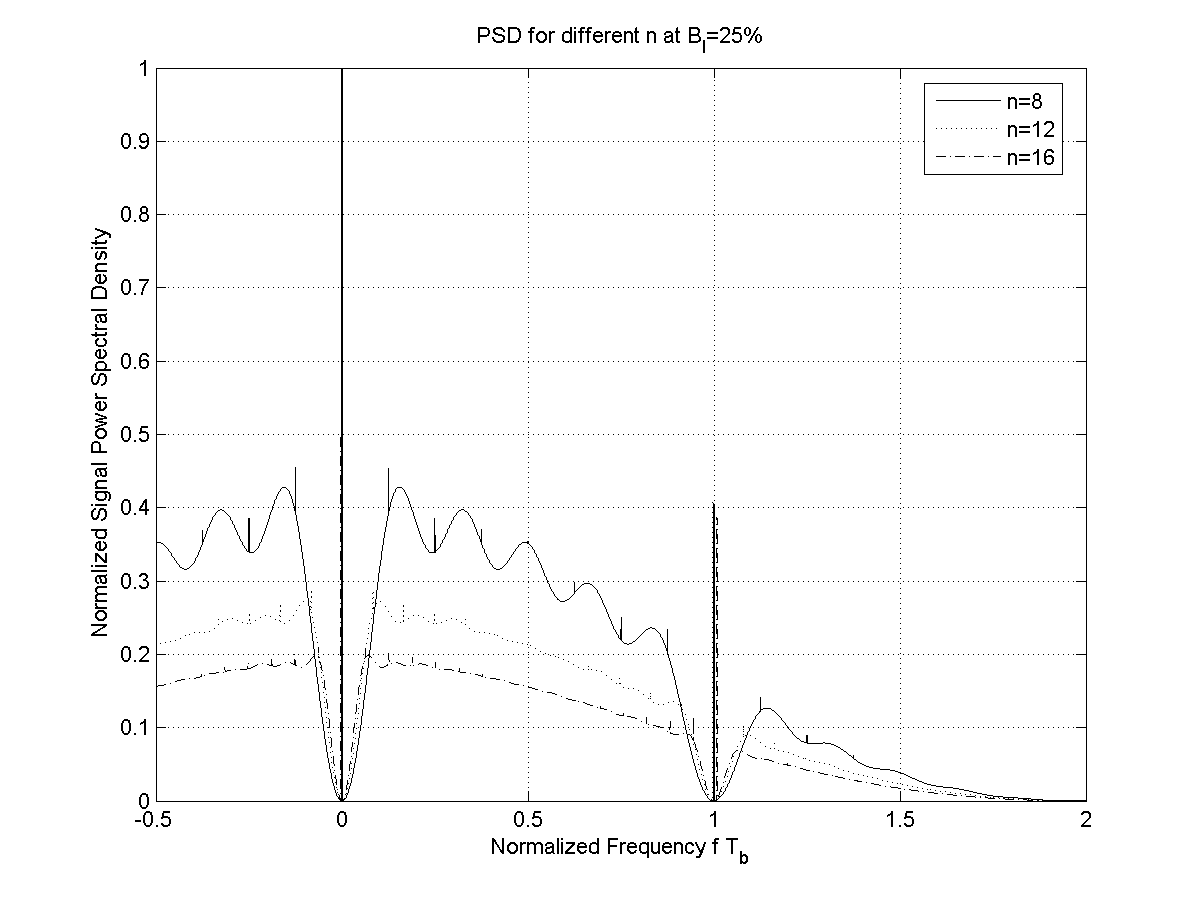
\includegraphics[width=\figwidth]{./Figures/252.png}  
%  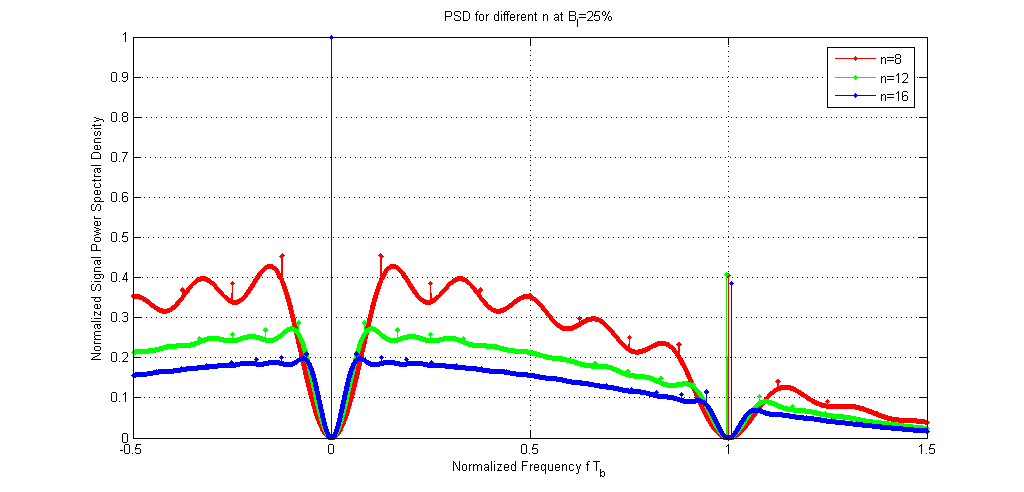
\includegraphics[width=\figwidth]{./Figures/25.png}   Colored Spectrum
  \caption[Effect of frame size on PSD]{Power spectral density for different values of frame size at fixed brightness index}
  \label {fig:fix_bi}
 \end{figure}

%\section{Effect Of Brightness Index $B_I$ On PSD}
\section{Effect Of Brightness Index On PSD}
Effect of brightness index with fixed frame size is plotted in figure \ref{fig:fix_n}. Brightness index has a profound effect on the DC spectral component. The plotted figure shows PSD for $n=8$ at $r=1,2~and~4$ respectively. The inspection of the spectrum at null frequency reveals that when the brightness index is doubled from 0.125 to 0.25,
increase in the corresponding DC component is four fold, from 0.125 to 0.5. Similarly increasing $B_I$ from 0.25 to 0.5, quadruples the DC component form 0.25 to 2.0. This behaviour is expected and confirms the squared relationship between signal voltage and its power. 


 \begin{figure}[hbtp]
  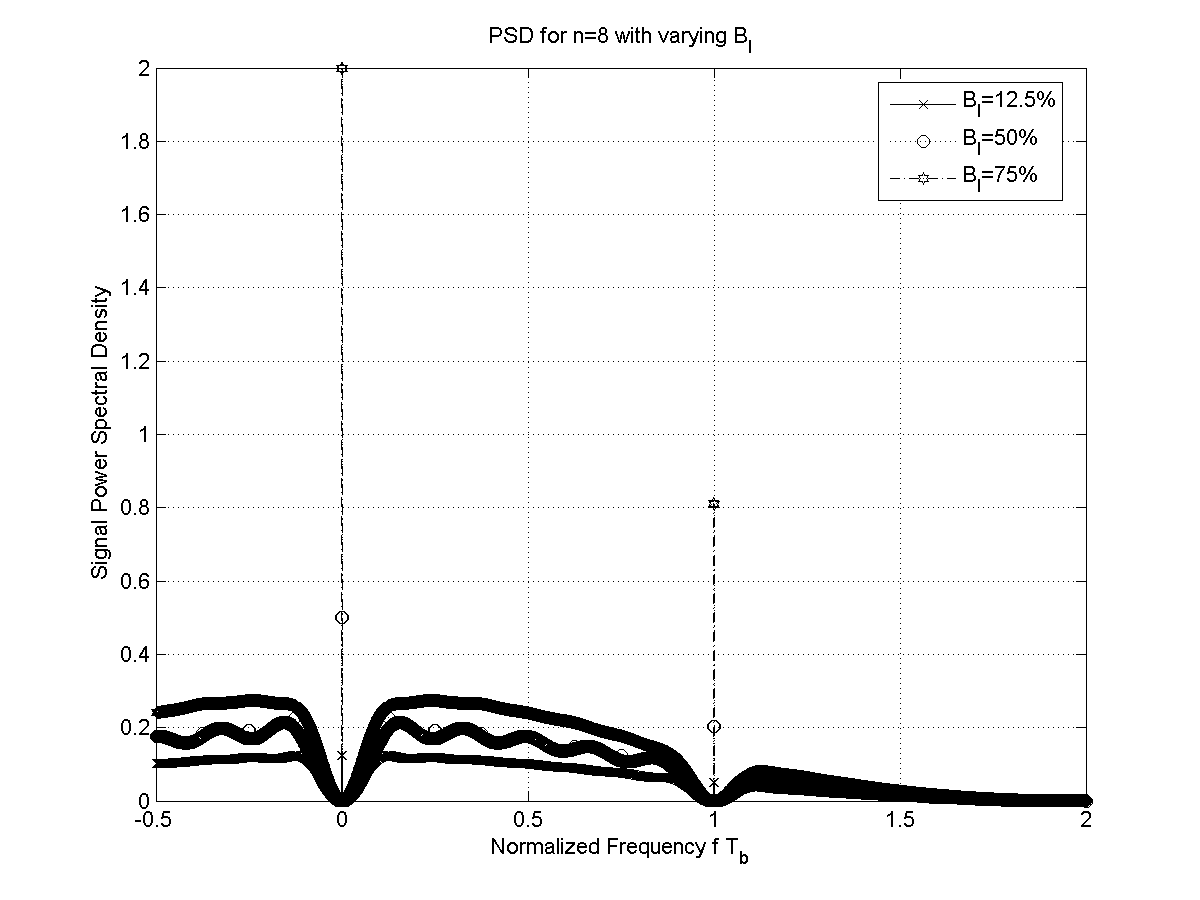
\includegraphics[width=\figwidth]{./Figures/fixN2.png}  
  \caption[Effect of brightness index on PSD]{Effect of changing brightness index on power spectral density, frame size being fixed}
  \label {fig:fix_n}
 \end{figure}

\section{Oscillations In The Spectrum}
%\sloppy
The continuous spectrum displays oscillatory behaviour which is significant at smaller frame size, $n$.  The number of oscillations increases with large codeword size with decreasing magnitude of oscillations. It is due to the influence of vector $V$ defined in (\ref{eq:vectorV}), reproduced below. Figure \ref{fig:OscilationWithN} shows the plot of continuous spectra for n= 2, 4, 8 and 16, evaluated to study the effect of oscillations. Though frame sizes of 2 and 4 provide poor brightness control resolution, the spectrum oscillations are much pronounced here. These graphs are plotted for fixed $r=1$ and PSDs are displaced vertically to separate apart for better inspection. It can be observed that the oscillations diminish for higher values of frame size. This is the same behaviour as adding more exponential terms to Fourier representation of a pulse smothers its time representation towards a better looking rectangle.

\[
	\mathbf{V}= \left[\mathbf{e}^{j\omega T_b}, \mathbf{e}^{j\omega 2T_b}, \cdots,\mathbf{e}^{j\omega nT_b}\right]
\]

 \begin{figure}[!hbtp]
  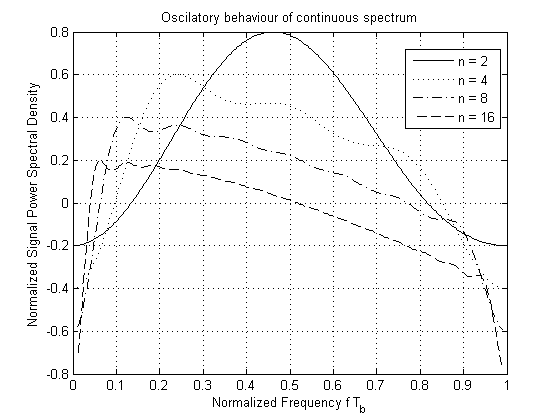
\includegraphics[width=\figwidth]{./Figures/OscilationWithN.png}  
  \caption{Oscillatory trend in spectral density}
  \label {fig:OscilationWithN}
 \end{figure}

The oscillations in continuous spectrum do not change much for a fixed frame size when brightness index is varied. It can be observed from the PSD for $n=10$ at different brightness indices, plotted in figure \ref{fig:OscilationWithR}. 

 \begin{figure}[!hbtp]
  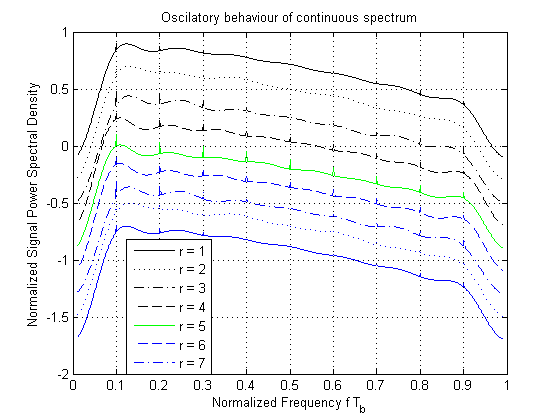
\includegraphics[width=\figwidth]{./Figures/OscilationWithR.png}  
  \caption[Effect of $B_I$ on oscilations in PSD]{Effect of brightness index on oscillations in power spectral density}
  \label {fig:OscilationWithR}
 \end{figure}

%Calculate fn

%>>>>>>>>>>>>>>>>>>>>>>>>>>>>>>>>>>
%
%<<<<<<<<<<<<<<<<<<<<<<<<<<<<<<<<<<

%<<<<<<<<<<<<<<<<<<<<<<<<<<<<<<<<<<